\documentclass[twocolumn,floatfix,aps,prd,nofootinbib]{revtex4-2}

\usepackage[utf8]{inputenc}
\usepackage[T1]{fontenc}
\usepackage{graphicx}
\usepackage{amssymb}
\usepackage{amsmath}
\usepackage{xcolor}
\usepackage{hyperref}
\usepackage{textcase}
\usepackage{placeins}
\usepackage[protrusion=true,expansion=false]{microtype}

\hypersetup{
    colorlinks=true,
    linkcolor=blue,
    filecolor=magenta,
    urlcolor=blue,
    citecolor=blue,
}
\urlstyle{same}
\emergencystretch=2em

\begin{document}

\title{\texorpdfstring{\MakeTextUppercase{Neural Spacetime Search with \texttt{GRTeclyn}: Geometry-First and Matter-First Baselines}}{Neural Spacetime Search with GRTeclyn: Geometry-First and Matter-First Baselines}}

\author{\MakeTextUppercase{Nikita M. Shirokov}}
\email{shirokov.nm@phystech.edu}
\affiliation{\textit{Independent Researcher, Moscow, Russia}}
\date{\today}

\begin{abstract}
We present a compact baseline for automated searches over dynamical spacetime
initial data.  A Python optimizer proposes low-dimensional parameters,
\texttt{GRTeclyn} evolves each candidate on GPU, and diagnostics score
constraint health, operational faster-than-light (FTL) benefit, stability, and
energy-condition cost.  The paper separates two regimes.  In the
\emph{geometry-first} regime the optimizer deforms the metric directly and uses
the constraints to infer the required matter.  This is cheap and has already
found a standing directional shortcut, but it does not supply the momentum
source needed for transport.  In the \emph{matter-first} regime the optimizer
proposes scalar-matter configurations and \texttt{GRTresna} solves the elliptic
constraints before \texttt{GRTeclyn} evolves the result.  This is the right path
toward physical searches, but current mixed exotic-lump MAP-Elites results
require a stricter post-load constraint gate because the matter stress tensor
solved by \texttt{GRTresna} need not equal the stress tensor evolved by
\texttt{GRTeclyn}.  We therefore treat the matter-first campaign as a promising
engineering milestone, not yet as a validated FTL metric discovery.
\end{abstract}

\maketitle

\section{Goal and Search Loop}
\label{sec:goal}

Most warp and wormhole metrics are hand-designed static ans\"atze.  Here the
metric is instead treated as the output of a black-box search over dynamical
3D initial data.  Throughout this paper ``FTL'' means an effective shortcut
through curved spacetime relative to a flat-spacetime control; it does not imply
local superluminal motion outside the local light cone.

The search problem is deliberately operational.  A useful candidate must be
non-trivial, approximately constraint-satisfying, dynamically stable for more
than a short smoke window, and faster than a flat control according to a probe
that is not merely reading off a gauge artifact.  The loop is
\[
\theta \rightarrow \hbox{initial data}
\rightarrow \texttt{GRTeclyn}
\rightarrow \hbox{diagnostics}
\rightarrow S(\theta),
\]
where $S$ is a bounded scalar score used by CMA-ES or MAP-Elites.  Health terms
are multiplied by a non-triviality gate so flat space cannot win simply because
it is stable.

\begin{figure*}[t]
\centering
\fbox{\begin{minipage}{0.94\textwidth}
\scriptsize
\textbf{Closed-loop evaluation}\\[0.35em]
\begin{tabular}{@{}c@{\ $\rightarrow$\ }c@{\ $\rightarrow$\ }c@{\ $\rightarrow$\ }c@{\ $\rightarrow$\ }c@{}}
\shortstack{candidate\\parameters} &
\shortstack{initial-data\\decoder} &
\shortstack{\texttt{GRTeclyn}\\GPU evolution} &
\shortstack{plotfile / small-data\\diagnostics} &
\shortstack{score and\\optimizer update}
\end{tabular}\\[0.35em]
The two decoders studied here are geometry-first recipes and matter-first
\texttt{GRTresna} elliptic solves.
\end{minipage}}
\caption{\textbf{Search loop.}  The optimizer sees only the scalar objective;
physics enters through the initial-data map and through post-evolution
diagnostics.}
\label{fig:closed_loop}
\end{figure*}

The score is not a single visual heuristic.  It combines four classes of
diagnostics.  First are shortcut indicators: axial null travel time
$F_{\rm null}$, proper-distance compression, throat pinching, and
Nat\'ario--Alcubierre expansion asymmetry.  Second is the operational probe
$F_{\rm op}$, an arrival-time comparison against a flat control on the same
grid.  Third are health terms: survival, Hamiltonian/momentum constraints,
lapse collapse, trapped-surface flags, and growth of $\chi$, $K$, and constraint
norms.  Fourth are risk terms: required negative energy, matter/effective energy
conditions, and tidal/curvature proxies.  The exact weights are not essential
for this paper; the key point is that a candidate must be both a shortcut and a
healthy evolved spacetime.

For an axial null probe on a conformally flat slice,
\begin{equation}
\begin{aligned}
T_{\rm curved} &=
\int_{-L}^{L}\frac{dx}{\alpha(x)\sqrt{\chi(x)}-\beta^x(x)},\\
F_{\rm null}&=\max\left(0,\frac{2L-T_{\rm curved}}{2L}\right).
\end{aligned}
\label{eq:null_shortcut}
\end{equation}
The final operational test compares arrival time to a flat control,
\begin{equation}
F_{\rm op}=\frac{t_B^{\rm flat}-t_B^{\rm curved}}{t_B^{\rm flat}},
\label{eq:f_op}
\end{equation}
and is accepted only with bounded constraints and no trapped-surface crossing.
The risk side tracks Hamiltonian/momentum norms, collapse indicators, geometry
growth, energy-condition margins, and required exotic energy
\begin{equation}
\rho_{\rm req}=
\frac{R+K^2-K_{ij}K^{ij}}{16\pi}.
\label{eq:rho_req}
\end{equation}
A non-triviality gate suppresses flat Minkowski space: health rewards are counted
only when the geometry has a real shortcut, curvature signal, asymmetry, or
exotic content.  This prevents the optimizer from selecting ``nothing happens''
as the most stable solution.

\section{Geometry-First Search}
\label{sec:geometry_first}

The first baseline asks the optimizer to propose geometric and gauge fields
directly.  For the conformally flat recipe, the Hamiltonian and momentum
constraints are read backwards:
\begin{equation}
\rho = \frac{R + K^2 - K_{ij}K^{ij}}{16\pi},\qquad
j_i = \frac{1}{8\pi}D_j(K^j_i-\delta^j_iK).
\label{eq:constraint_sources}
\end{equation}
Regions with $\rho<0$ become an exotic-matter cost.  In the simplest radial
recipe,
\begin{equation}
q(r)=q_\infty+\sum_n a_n B_n(r),
\end{equation}
where $q$ denotes $\chi$, lapse, shift, or $K$.  Angular modes are then added in
the gauge sector.  This is computationally cheap because it avoids a 3D
elliptic solve, but it has a hard limitation: with $K=\mathrm{const}$ and
$\Pi=0$ the momentum density vanishes.  The recipe can bend space into a lens,
but it cannot provide a co-moving matter current.

\subsection{Validated Baseline Result}

The best geometry-first outcome is a standing Alcubierre-like dipole.  The
search found non-spherical gauge/geometric structure with a localized exotic
core rather than a translating bubble.  A representative promoted candidate,
\texttt{eval\_000188}, was replayed to $t=16$ at $N_{\rm full}=192$.  It retained
a weak evolved operational shortcut,
\[
F_{\rm op}^{\rm ev}=5.6\times10^{-3},
\]
with decreasing constraint norms
$\|H\|_{L^2}:1.1\times10^{-3}\rightarrow4.2\times10^{-4}$ and final
$\|M\|_{L^2}=3.6\times10^{-5}$.  The required negative energy stayed localized,
\[
\int \rho_-\,dV\simeq0.13,\qquad
\min\rho_{\rm req}\simeq -10^{-3}.
\]
This is a useful automated-discovery baseline: the search can identify a
structured, low-exotic shortcut geometry that survives longer than the smoke
window.  It is not a transport metric.  The structure stands and relaxes rather
than carrying a passenger region across the grid.

\begin{figure}[tbp]
\centering

\includegraphics[width=\columnwidth]{articlepictures/chi_vs_rho_req.png}
\caption{\textbf{Geometry-first dipole.}  The validated candidate is a static
exotic lens: the compression lobe in $\chi$ is supported by a localized negative
required energy density.}
\label{fig:rho_req}
\end{figure}

\begin{figure}[tbp]
\centering
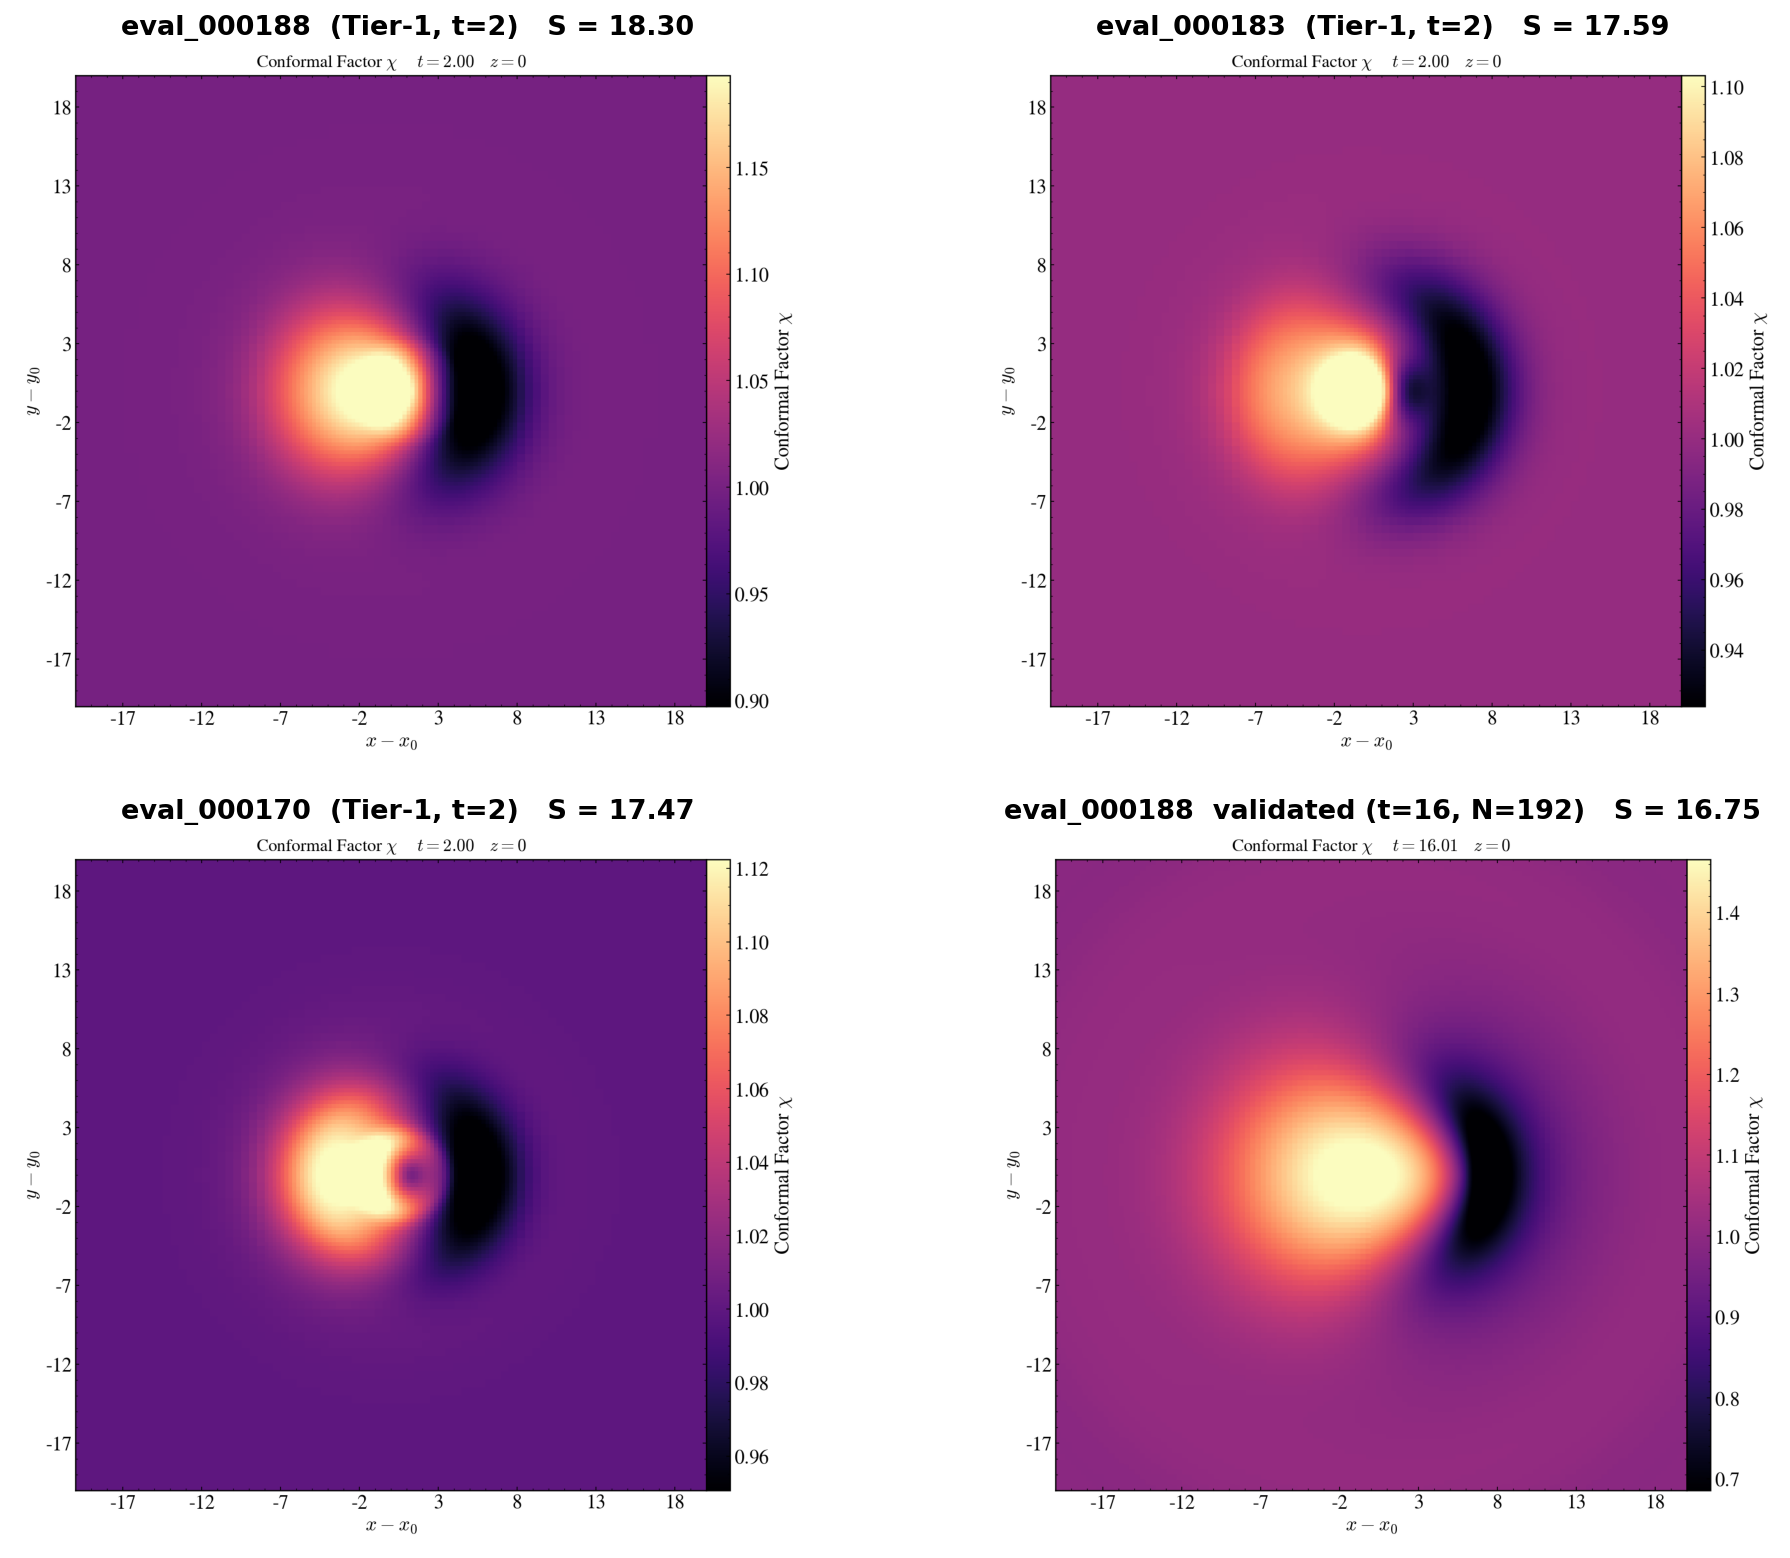
\includegraphics[width=\columnwidth]{articlepictures/chi_tiles.png}
\caption{\textbf{Directional geometry-first candidates.}  The top candidates
share the same standing expand-behind/compress-ahead polarity.  This is the
geometry a warp channel needs, but not the matter current needed to move it.}
\label{fig:chi_tiles}
\end{figure}

The lesson is clear.  Geometry-first search is a fast way to discover useful
geometric motifs and to test scoring diagnostics, but the optimizer naturally
prefers a cheap stationary lens over a harder translating bubble.  A transport
metric needs a sustained momentum density $j_i$, because $G_{0i}=8\pi j_i$ ties
matter current to the frame-dragging shift.

\section{Matter-First Search}
\label{sec:matter_first}

The matter-first route inverts the map.  The optimizer proposes matter; an
elliptic solver returns the compatible geometry.  For scalar matter,
\begin{equation}
\rho=\frac12\psi^{-4}|\tilde\nabla\phi|^2+\frac12\Pi^2+V(\phi),
\qquad
S_i=-\Pi\,\partial_i\phi .
\label{eq:scalar_sources}
\end{equation}
\texttt{GRTresna} solves the Hamiltonian and momentum constraints for the
conformal factor and longitudinal extrinsic curvature, writes a
\texttt{.gridinit} file, and \texttt{GRTeclyn} evolves it.  This adds the missing
ingredient from Sec.~\ref{sec:geometry_first}: searchable momentum-carrying
matter.

\begin{figure*}[t]
\centering
\fbox{\begin{minipage}{0.94\textwidth}
\small
\textbf{Matter-first discovery stages}\\[0.35em]
\begin{tabular}{@{}c@{\ $\rightarrow$\ }c@{\ $\rightarrow$\ }c@{\ $\rightarrow$\ }c@{}}
16D shell vector &
MAP-Elites archive &
optional CMA-ES refinement &
high-resolution promotion / validation
\end{tabular}\\[0.35em]
The shell vector expands to five Fibonacci-distributed scalar clouds.  MAP-Elites
keeps diverse families by descriptor cell instead of collapsing to one scalar
optimum.
\end{minipage}}
\caption{\textbf{Shell discovery workflow.}  This is the compact form of the
README pipeline: broad quality-diversity search, optional local refinement, and
fresh high-resolution replay.}
\label{fig:shell_workflow}
\end{figure*}

\begin{figure*}[t]
\centering
\fbox{\begin{minipage}{0.94\textwidth}
\small
\textbf{Per-candidate matter-first loop}\\[0.35em]
\begin{tabular}{@{}c@{\ $\rightarrow$\ }c@{\ $\rightarrow$\ }c@{\ $\rightarrow$\ }c@{\ $\rightarrow$\ }c@{\ $\rightarrow$\ }c@{}}
sample shell params &
\texttt{GRTresna} solve &
Ham/Mom gate &
\texttt{.gridinit} &
\texttt{GRTeclyn} evolve &
score/archive
\end{tabular}\\[0.35em]
The missing production gate is a post-load \texttt{GRTeclyn} constraint check
using the matter model that is actually evolved.
\end{minipage}}
\caption{\textbf{Matter-first evaluation.}  GRTresna convergence is necessary
but not sufficient: the loaded state must also satisfy the constraints under the
GRTeclyn evolution stress tensor.}
\label{fig:per_eval}
\end{figure*}

\subsection{Shell Parameterization and MAP-Elites}

The current discovery ansatz uses a 16-dimensional shell vector.  It places a
small number of scalar clouds on a Fibonacci lattice over the sphere, rotates
the lattice by a searched orientation axis, and assigns toroidal, poloidal, and
radial velocity components.  Low-order dipole/quadrupole modulations control
matter asymmetry, while an exotic wedge selects where negative-energy support is
attempted.  MAP-Elites is used because preserving diverse mechanism families is
more valuable here than only optimizing a single scalar score.

The recent shell campaign produced strong operational signals in the search
logs, including promoted candidates with large $F_{\rm op}^{\rm ev}$ after
longer replay.  These are important engineering signals: the optimizer,
elliptic solver, GPU evolution, plotfile consumption, and archive machinery can
all run at scale.  They are not yet a validated physical result for the mixed
exotic-lump search space.

\subsection{Current Trust Issue}
\label{sec:trust_issue}

The reason is a matter-model mismatch.  \texttt{GRTresna} may solve a source
that is not the same stress-energy \texttt{GRTeclyn} evolves after loading
\texttt{.gridinit}.  Three effects matter.

First, exotic lumps in \texttt{GRTresna} enter the source as independent phantom
components, with their kinetic and momentum terms multiplied by a negative sign.
The written \texttt{phi} and \texttt{Pi} fields do not carry that sign.  If
\texttt{GRTeclyn} evolves the combined field as a canonical scalar, the local
Hamiltonian source has the wrong sign in exotic regions.

Second, the solved source treats lumps as independent fields and drops
inter-lump cross terms.  The evolved single scalar contains the combined field,
so $|\nabla\sum_k\phi_k|^2$ includes cross terms wherever clouds overlap.

Third, the solver source can include a mass potential while the current
\texttt{GRTeclyn} default potential is zero.  Thus a small
\texttt{GRTresna} Hamiltonian residual certifies the elliptic solve, not
necessarily the state that is actually evolved.

The practical criterion is therefore stricter:
\begin{quote}
A matter-first candidate is trusted only if the loaded \texttt{GRTeclyn} state
passes the Hamiltonian and momentum constraints at $t=0$ using the same matter
model that will be evolved, and then remains bounded under replay.
\end{quote}
Until that gate is added and applied to the shell archive, the MAP-Elites
numbers should be reported as promising search signals rather than as evidence
for a validated FTL geometry.

\section{Path to a Trustworthy Matter-First Campaign}
\label{sec:path}

The next campaign should be organized around falsification rather than score
maximization.  The required steps are short and concrete.

\paragraph{Post-load constraint gate.}
After \texttt{GRTresna} writes \texttt{.gridinit}, load the file into
\texttt{GRTeclyn}, compute $H$ and $M_i$ with the actual evolution matter model,
and reject candidates before GPU evolution if the $t=0$ residual is large.  This
is the missing gate in Fig.~\ref{fig:per_eval}.

\paragraph{Representable matter.}
Either restrict the search to matter that a single evolved scalar can represent
(for example all-canonical or all-phantom, matched potential, limited overlap),
or promote the evolution model to the same independent-field stress tensor that
\texttt{GRTresna} solved.  A frozen prescribed source should not be used for
physics claims, because it repeats the known failure mode $G_{ab}\neq8\pi T_{ab}$
as soon as the geometry evolves.

\paragraph{Transport objective.}
The current objective rewards the existence of a shortcut on a slice.  A warp
metric needs a co-moving worldtube: a localized passenger region moving a finite
distance while the surrounding geometry is approximately stationary in its own
frame.  The score should require this condition, otherwise the optimizer will
continue to prefer static lenses.

\paragraph{Resolution and observer checks.}
Any surviving candidate must be replayed on a resolution ladder and evaluated
with observer-robust energy conditions, not only matter-sector diagnostics.
The target validation ladder is: constructed, non-trivial, post-load
constraint-clean, operational, persistent, observer-robust, resolution-converged,
and analytically extractable.

\paragraph{Analytical extraction.}
A numerical elite is only a coefficient vector.  The final step is fitting a
closed-form metric or matter profile, re-solving the constraints from that form,
and replaying it.  This is what turns the search result into a checkable
spacetime rather than an isolated grid artifact.

\section{Conclusion}

The geometry-first search is a useful baseline: it is fast, debugs the scoring
pipeline, and has found a clean standing shortcut supported by a localized
exotic core.  Its limitation is also decisive: it does not supply the sustained
momentum source needed for transport.  Matter-first search with \texttt{GRTresna}
is the better route because it exposes momentum-carrying matter and solves the
constraints before evolution.  However, the current mixed exotic-lump
MAP-Elites results should be treated conservatively until the post-load
\texttt{GRTeclyn} constraint gate and matched matter model are in place.  The
near-term goal is therefore not to claim a new FTL metric, but to turn the
matter-first pipeline into a falsifiable and constraint-clean discovery engine.

\section{Update: Resolution of the Matter-First Trust Issue}
\label{sec:update_fixed}

The blocking steps identified in Sec.~\ref{sec:trust_issue} and
Sec.~\ref{sec:path} have now been implemented and validated end to end.  The
matter-model mismatch that previously invalidated the loaded \texttt{GRTeclyn}
state has been removed, so matter-first candidates are now constraint-clean at
$t=0$ under the same stress-energy that is evolved.

\paragraph{Matched independent-field matter (fixed).}
\texttt{GRTeclyn} now evolves a dedicated independent signed-scalar matter model
(\texttt{GRTresnaIndependentScalars}) that mirrors the \texttt{GRTresna} source:
each lump carries its own sign, kinetic and momentum terms are summed
per-lump, and no inter-lump cross terms are introduced.  This directly resolves
the first two effects of Sec.~\ref{sec:trust_issue} (the wrong-sign exotic
source and the spurious $|\nabla\sum_k\phi_k|^2$ cross terms).  The
\texttt{.gridinit} writer now also carries the per-lump $\phi_k,\Pi_k$ channels
and a matter-layout metadata record so the evolution reconstructs the solved
fields exactly.

\paragraph{Matched potential (fixed).}
The evolution potential is set to the mass-matched form
$V(\phi)=\tfrac{1}{2}m^2\phi^2$ using the same scalar mass as the solve, so the
third effect of Sec.~\ref{sec:trust_issue}---a solver/evolution potential
mismatch---no longer applies.

\paragraph{Post-load constraint gate (fixed).}
The missing gate of Fig.~\ref{fig:per_eval} is now in place.  After
\texttt{GRTresna} writes \texttt{.gridinit}, the file is loaded into
\texttt{GRTeclyn}, $H$ and $M_i$ are evaluated with the actual evolution matter
model, and candidates whose $t=0$ residual exceeds a threshold
($L^2_{H},L^2_{M}\le 10^{-2}$ by default) are rejected before GPU evolution.
This gate is mandatory in both the CMA-ES and MAP-Elites loops.

\paragraph{Robust exotic solves (fixed).}
Configurations containing negative-energy lumps automatically switch to the
$K=0$ maximal-slicing (York--Lichnerowicz) solver with Newton under-relaxation
and a conformal-factor floor, instead of the default
$K=\mathrm{sign}\sqrt{24\pi G\rho+\dots}$ ansatz that is imaginary where
$\rho<0$.  This removes the spurious \texttt{NaN} rejections that previously
afflicted exotic candidates.

\paragraph{Validation.}
End-to-end smokes covering canonical, exotic, and mixed overlapping-shell
configurations pass: the \texttt{GRTresna} solves remain finite, the
29-component \texttt{.gridinit} loads correctly, and the post-load constraints
are small ($L^2_{H}\approx4\times10^{-3}$, $L^2_{M}\approx2\times10^{-4}$).
Surviving evolved candidates report \texttt{constraint\_health}$\approx0.95$,
\texttt{survival}$=1$, and satisfy the averaged null energy diagnostic over the
sampled tube.

\paragraph{Scope of the claim.}
These fixes establish \emph{physical self-consistency}: a surviving candidate is
now a genuine, constraint-satisfying solution of the Einstein equations rather
than a state that violates $G_{ab}=8\pi T_{ab}$ on load.  They do \emph{not} by
themselves establish a transport-capable (operational-FTL) geometry; that
remains the objective of the search campaign (Sec.~\ref{sec:path}, transport
objective and observer/resolution checks).  In short, the constraint-validity
prerequisites of the matter-first pipeline are resolved, and the remaining work
is the physics search for an operational, observer-robust, resolution-converged
elite.

\begin{thebibliography}{9}

\bibitem{alexander2026albert}
S.~Alexander, B.~Bradley, L.~Gouskos, and C.~Niu,
\newblock ``Autonomous Discovery of Particle Physics Theories from Experimental Data,''
\newblock arXiv:2603.28935 [hep-ph] (2026).

\bibitem{qiu2026collideragent}
S.~Qiu, Z.~Cai, J.~Wei, Z.~Li, Y.~Yin, Q.-H.~Cao, C.~Liu, M.-x.~Luo, X.-B.~Yuan, and H.~X.~Zhu,
\newblock ``An End-to-end Architecture for Collider Physics and Beyond,''
\newblock arXiv:2603.14553 [hep-ph] (2026).

\bibitem{halverson2019branes}
J.~Halverson, B.~Nelson, and F.~Ruehle,
\newblock ``Branes with Brains: Exploring String Vacua with Deep Reinforcement Learning,''
\newblock JHEP \textbf{06}, 003 (2019), arXiv:1903.11616 [hep-th].

\bibitem{han2025physagent}
X.-Q.~Han, Z.-F.~Gao, P.-J.~Guo, and Z.-Y.~Lu,
\newblock ``PhysAgent: A Multi-Agent Approach to Automated Discovery of Physical Laws,''
\newblock arXiv preprint (2025).

\bibitem{helmerich2024warpfactory}
C.~Helmerich, J.~Fuchs, A.~Bobrick, L.~Sellers, B.~Melcher, and G.~Martire,
\newblock ``Analyzing Warp Drive Spacetimes with Warp Factory,''
\newblock Class.\ Quantum Grav.\ (2024), arXiv:2404.03095 [gr-qc].

\bibitem{le2026warpax}
A.~T.~Le,
\newblock ``Observer-robust energy condition verification for warp drive spacetimes,''
\newblock arXiv:2602.18023 [gr-qc] (2026).

\bibitem{lousto2006fourth}
C.~O.~Lousto,
\newblock ``A time-domain fourth-order-convergent numerical algorithm to integrate black hole perturbations in the extreme-mass-ratio limit,''
\newblock Class.\ Quantum Grav.\ \textbf{22}, S543 (2005), arXiv:gr-qc/0503001.

\bibitem{li2023pinn}
Z.-H.~Li, C.-Q.~Li, and L.-G.~Pang,
\newblock ``Solving Einstein equations using deep learning,''
\newblock arXiv:2309.07397 [gr-qc] (2023).

\end{thebibliography}

\end{document}
